\begin{theo}[Convexity for $C^1$ functions]{ConvexityC1}
    \begin{minipage}{0.60\textwidth}
        Assume that $f: \ \Omega \rightarrow \R$ is continuously differentiable and $\Omega$ is convex. Then holds that $f$ is convex if and only if 
        \begin{equation*}
            \forall x,y \in \Omega: \ f(y) \geq f(x) + \nabla f(x)^T(y-x)
        \end{equation*}
        i\@.e\@. tangents lie below the graph.
    \end{minipage}
    \begin{minipage}{0.3\textwidth}
        \begin{center}
            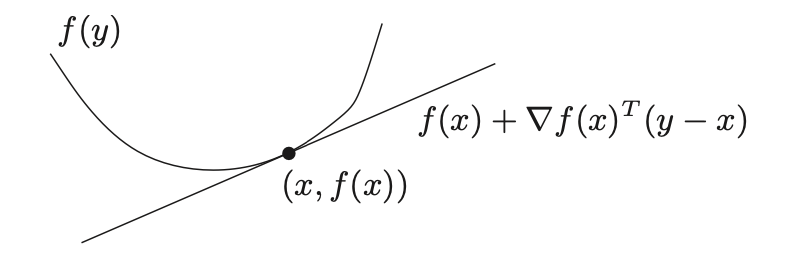
\includegraphics[scale = 0.45]{Images/Fundamental/C1Convexity.png}
        \end{center}
    \end{minipage}
\end{theo}

\begin{prf}[Convexity for $C^1$ functions]{prfConvexityC1}
    ``$\Rightarrow$'': Due to convexity of $f$ holds for given $x,y \in \Omega$  and for any $\lambda \in [0,1]$ that
    \begin{equation*}
        f(x + \lambda(y-x)) - f(x) \leq \lambda(f(y) - f(x)).
    \end{equation*}
    and therefore that 
    \begin{equation*}
        \nabla f(x)^T(y-x) 
            = \lim_{\lambda \rightarrow 0}  \frac{f(x + \lambda(y-x)) - f(x)}{\lambda}
            \leq \frac{f(y) - f(x)}{y-x}.
    \end{equation*}

    ``$\Leftarrow$'': To prove that $z = x + \lambda(y-x) = (1-\lambda)x + \lambda y$ holds that $f(z) \leq (1-\lambda)f(x) + \lambda f(y)$, we can use the equation from Theorem~\ref*{ConvexityC1} twice to get
    \begin{equation*}
        f(x) \geq f(z) + \nabla f(z)^T(x-z) \ \ \text{and} \ \ f(y) \geq f(z) + \nabla f(z)^T(y-z),
    \end{equation*}
    which yield, when weighted with $(1-\lambda)$ and $\lambda$ respectively, that
    \begin{equation*}
        (1-\lambda)f(x) + \lambda f(y) \geq f(z) + \nabla f(z)^T \underset{= 0}{\underbrace{\left[(1-\lambda)(x-z) + \lambda(y-z)\right]}}
    \end{equation*}
    \vspace{-0.75cm}
\end{prf}

\begin{theo}[Convexity of Sublevel subsets]{ConvexitySublevelSubset}
    \vspace*{-0.5cm}
    \begin{minipage}{0.58\textwidth}
        The sublevel set 
        \begin{equation*}
            \{ \ x \in \Omega \ | \ f(x) \leq c \ \}
        \end{equation*} 
        of a convex function $f: \Omega \rightarrow \R$ with respect to any constant $c \in \R$ is convex. 
    \end{minipage}
    \begin{minipage}{0.38\textwidth}
        \begin{center}
            \vspace*{0.5cm}
            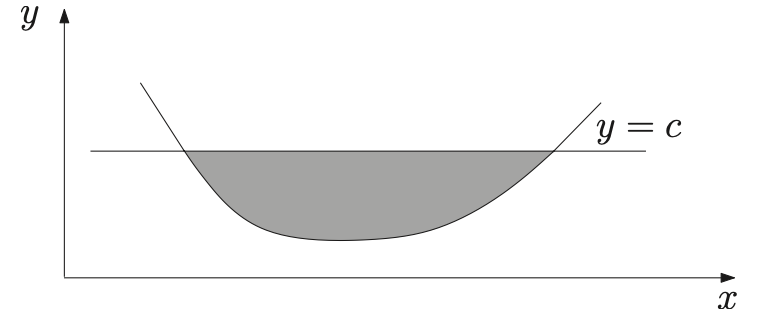
\includegraphics[scale = 0.475]{Images/Fundamental/ConvexSubset.png}
        \end{center}
    \end{minipage}
    \vspace{-0.3cm}
\end{theo}

\begin{prf}[Convexity of Sublevel subsets]{prfConvexitySublevelSubset}
    If $f(x) \leq c$ and $f(y) \leq c$, then for any $\lambda \in [0,1]$ holds also 
    \begin{equation*}
        f((1-\lambda)x + \lambda y) \leq (1-\lambda)f(x) + \lambda f(y) \leq \underset{= c}{\underbrace{(1-\lambda)c + \lambda c}}.
    \end{equation*}
    \vspace*{-0.7cm}
\end{prf}

\begin{pro}[Convexity perserving operations on convex sets]{ConvexityPreservingOperations}
    The following operations preserve convexity of a set:
    \begin{enumerate}
        \item The intersection of finitely or infinitely many convex sets is convex.
        \item Affine image: if $\Omega$ is convex, then for $A \in \R^{m \times n}$, $b \in \R^m$ also the set $A\Omega + b = \{ y \in \R^m \ | \ \exists x \in \Omega : y = Ax + b \}$ is convex.
        \item Affine pre-image: if $\Omega$ is convex, then for $A \in \R^{n \times m}$, $b \in \R^n$ also the set $\{ z \in \R^m \ | \ Az + b \in \Omega \}$ is convex.
    \end{enumerate}
\end{pro}